% begin module derivative-sine
\begin{frame}
\begin{align*}
\text{Let}\quad f(x) & = \sin x. \\
\uncover<2->{%
\text{Then}\quad f'(x) & =  %
\lim_{h\rightarrow 0}\frac{f(x+h)-f(x)}{h}%
}%
\uncover<3->{%
 = \lim_{h\rightarrow 0}\frac{\alertNoH{ 4}{\sin (x+h)}-\sin x}{h}%
}\\%
& \uncover<4->{ = }  %
\uncover<4->{%
\lim_{h\rightarrow 0}\frac{\alertNoH{ 4}{ \alertNoH{5}{\sin x \cos h} + \alertNoH{6}{\cos x \sin h}} \alertNoH{5}{- \sin x}}{h}%
}\\%
& \uncover<5->{ = }  %
\uncover<5->{%
\lim_{h\rightarrow 0}\left( \frac{ \alertNoH{5}{\alertNoH{7}{ \sin x} \cos h - \alertNoH{7}{\sin x}}}{h} + \frac{\alertNoH{6}{\cos x \sin h}}{h}\right) %
}\\%
& \uncover<7->{ = }  %
\uncover<7->{%
\lim_{h\rightarrow 0}\left( \alertNoH{7}{\sin x}\left( \frac{\cos h - 1}{h}\right) + \cos x\left( \frac{\sin h}{h}\right) \right) %
}\\%
& \uncover<8->{ = }  %
\uncover<8->{%
\alertNoH{ 9-10}{\lim_{h\rightarrow 0} \sin x}\cdot \alertNoH{ 13}{\lim_{h\rightarrow 0}\left( \frac{\cos h - 1}{h}\right)} + \alertNoH{ 11-12}{\lim_{h\rightarrow 0}\cos x}\cdot \alertNoH{ 13}{\lim_{h\rightarrow 0}  \left(\frac{\sin h}{h}\right)}  %
}\\%
& \uncover<9->{ = }  %
\uncover<9->{%
\alertNoH{ 9-10}{\fcAnswer{10}{\sin x}}\cdot \alertNoH{ 13}{\lim_{h\rightarrow 0} \left(\frac{\cos h - 1}{h}\right)} + \alertNoH{ 11-12}{\fcAnswerUncover{9}{12}{\cos x}}\cdot \alertNoH{ 13}{\lim_{h\rightarrow 0}  \left(\frac{\sin h}{h}\right)}  %
}%
\end{align*}
\uncover<13->{%
We need to do more work to find the other two limits.

}%
\end{frame}
\begin{frame}
\begin{columns}[c]
\column{.6\textwidth}
\[
\text{Claim:}\quad \lim_{\theta \rightarrow 0}\frac{\sin \theta }{\theta} = 1
\]
Suppose $\alertNoH{18}{ \alertNoH{9}{0 < \theta} < \frac{\pi}{2}}$.  \uncover<2->{\alertNoH{2}{Write $\sin \theta$ using ratios of side lengths of a triangle.}}
\column{.4\textwidth}
\psset{xunit=1.2cm, yunit=1.2cm}
\begin{pspicture}(-0.3, -0.3)(3.4,2)%
\psframe*[linecolor=white](-0.3,-0.3)(3.4,2)%
\tiny%
\psline[linecolor=gray!1](3.2, 2)(3.25, 2.05)%
\only<1-4, 8-10,12->{\psplot[linewidth=1pt]{2.598076211}{3}{9 x x mul sub sqrt}}%
\only<5-7,8,11,16>{\psplot[linecolor=red, linewidth=1.5pt] {2.598076211}{3}{9 x x mul sub sqrt}}%
\psline[linewidth=1pt](0,0)(3,0)%
\uncover<handout:0|14,15>{\psline[linecolor=red, linewidth=1.5pt](0,0)(3,0)}%
\psline[linewidth=1pt](0,0)(2.598076211,1.5)%
\only<3>{\psline[linecolor=red, linewidth=1.5pt](0,0)(2.598076211,1.5)}%
\psline[linewidth=1pt](-0.05,0.08660254)(2.548076211,1.58660254)%
\psline[linewidth=1pt](-0.025, 0.04330127) (-0.075, 0.12990381)%
\psline[linewidth=1pt](2.573076211, 1.54330127) (2.523076211, 1.62990381)%
\rput[b](1.25,0.9){\alertNoH{15}{$1$}}%
\only<1-2, 5-7>{ %line BC
\psline[linewidth=1pt](2.598076211,0)(2.598076211,1.5)
\psline[linewidth=1pt](2.498076211,0)(2.498076211,0.1)(2.598076211,0.1)}%
\only<3-4,8>{ % line BC
\psline[linecolor=red, linewidth=1.5pt](2.598076211,0)(2.598076211,1.5)
\psline[linecolor=red, linewidth=1pt] (2.498076211,0)(2.498076211,0.1)(2.598076211,0.1)}%
\only<9->{ % line BC
\psline[linecolor=gray, linewidth=1pt](2.598076211, 0)(2.598076211, 1.5)%
\psline[linecolor=gray, linewidth=1pt] (2.498076211, 0)(2.498076211, 0.1)(2.598076211,0.1)}%
\only<4-5>{ %line AB
\psline[linecolor=red, linewidth=1.5pt](2.598076211,1.5)(3,0)}%
\only<6-7>{ %line AB
\psline[linewidth=1pt](2.598076211,1.5)(3,0)}%
\only<8->{ %line AB
\psline[linecolor=gray, linewidth=1pt] (2.598076211,1.5)(3,0)}%
\only<11-12>{ % line BD
\psline[linewidth=1.5pt, linecolor=red] (2.598076211,1.5)(3, 0.866025404)}%
\only<13->{ % line BD
\psline[linewidth=1pt](2.598076211,1.5)(3,0.866025404)}%
\only<11, 13-14,16>{ %line DA
\psline[linewidth=1.5pt, linecolor=red](3, 0.866025404)(3,0)%
\psline[linewidth=1pt, linecolor=red](2.9,0)(2.9,0.1)(3,0.1)%
\rput[l](3.1,0.866025404){$D$}}%
\only<12, 15,17->{ %line DA
\psline[linewidth=1pt](3, 0.866025404)(3,0)%
\psline[linewidth=1pt, linecolor=gray](2.9,0)(2.9,0.1)(3,0.1)%
\rput[l](3.1,0.866025404){$D$}}%
%\only<12>{ %line BE
%\psline[linewidth=1.5pt, linecolor=red](2.598076211, 1.5)(3,1.732050808)%
%\psline[linewidth=1pt, linecolor=red](2.684678752, 1.55) (2.734678752,1.46339746) (2.648076211,1.41339746)}%
\only<12->{ %line BE
\psline[linewidth=1pt](2.598076211,1.5)(3,1.732050808)%
\psline[linewidth=1pt](2.684678752, 1.55) (2.734678752, 1.46339746) (2.648076211, 1.41339746)}%
\only<12-14,16>{ %line DE
\psline[linewidth=1.5pt, linecolor=red](3, 1.732050808)(3, 0.866025404)%
\rput[l](3.1,1.732050808){$E$}}%
\only<15,17->{ %line DE
\psline[linewidth=1pt](3, 1.732050808)(3,0.866025404)%
\rput[l](3.1, 1.732050808){$E$}}%
\uncover<7-10>{\rput[l](2.95,0.8){$\alertNoH{7}{\theta}$}}%
\rput[lb](0.3, 0.02){\alertNoH{7}{$\theta$}}%
\psarc[linecolor=red](0,0){0.29}{0}{30}%
\rput[tr] (-0.1,-0.1){$O$}%
\rput[t] (2.598076211,-0.1){$C$}%
\rput[t] (3,-0.1){$A$}%
\rput[b](2.598076211,1.6){$B$}%
\end{pspicture}
%\ \only<handout:0| -3>{%
%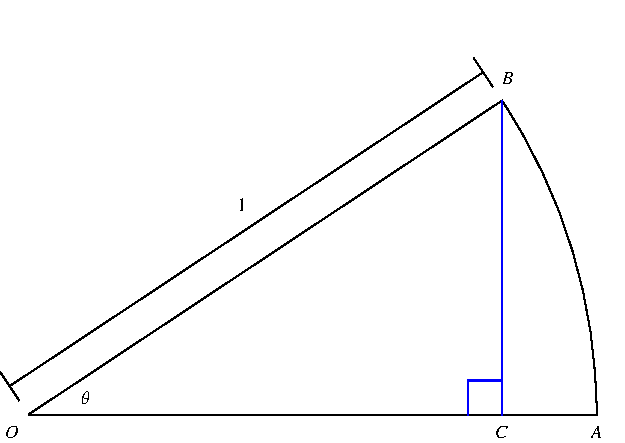
\includegraphics[width=4.5cm]{derivatives-trig/pictures/03-04-proofa.pdf}%
%}%
%\only<handout:0| 4-9>{%
%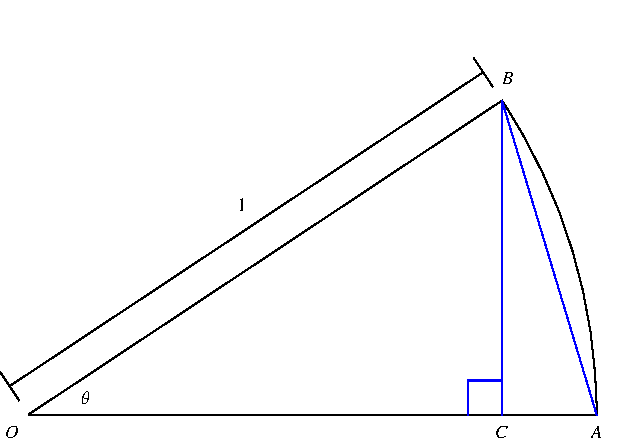
\includegraphics[width=4.5cm]{derivatives-trig/pictures/03-04-proofb.pdf}%
%}%
%\only<handout:0| 10>{%
%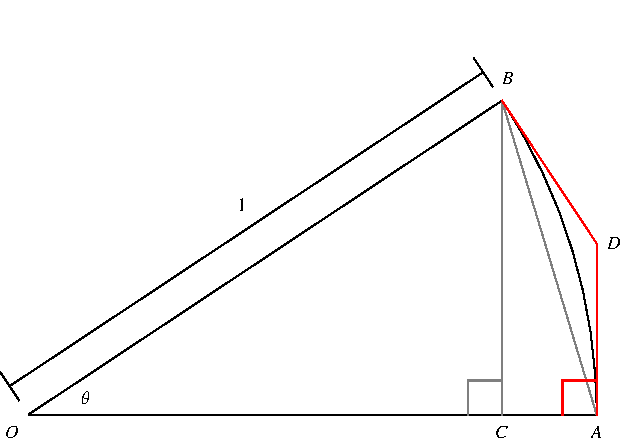
\includegraphics[width=4.5cm]{derivatives-trig/pictures/03-04-proofc.pdf}%
%}%
%\only<11->{%
%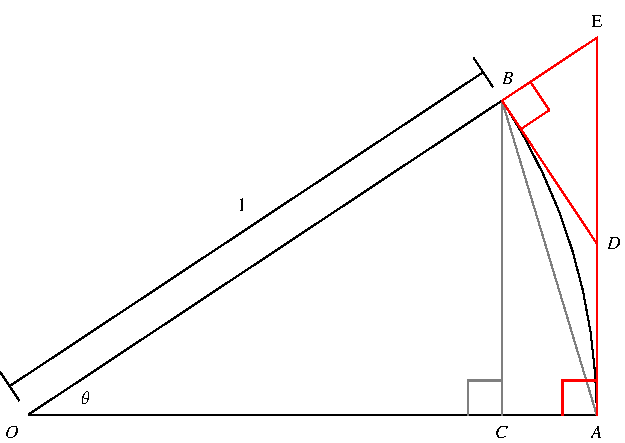
\includegraphics[width=4.5cm]{derivatives-trig/pictures/03-04-proofd.pdf}%
%}%

\end{columns}
\[
\uncover<2->{%
\alertNoH{ 2-3}{%
\alertNoH{8}{\sin \theta }= \fcAnswer{3}{\frac{|BC|}{ |OB|} = \alertNoH{4}{|BC|} } %
}%
}%
\uncover<4->{%
\alertNoH{4}{<\alertNoH{5}{|AB|}}%
}%
\uncover<5->{%
 \alertNoH{5,8}{<} \alertNoH{ 5-7}{\text{arc} AB \uncover<6->{ = } \fcAnswer{7}{\alertNoH{8}{\theta}}}%
}%
\]
\uncover<8->{%
Therefore $\alertNoH{8}{\sin\theta <\alertNoH{9}{\theta}}$ \uncover<9->{and therefore $\alertNoH{ 21}{\frac{\sin \theta}{\alertNoH{9}{\theta}} < 1}$.}%
}%
\abovedisplayskip=0pt
\belowdisplayskip=0pt
\begin{align*}
\uncover<10->{%
\alertNoH{16}{\theta} =\alertNoH{11}{ \text{arc} AB} %
}%
& \uncover<11->{ < }  %
\uncover<11->{%
\alertNoH{11}{|AD|} + \alertNoH{ 11,12}{|DB|}%
}  \uncover<12->{ \alertNoH{16}{<} }  \uncover<12->{%
\alertNoH{13}{|AD| + \alertNoH{ 12}{|DE|}}%
}\\%
& \uncover<13->{\alertNoH{13}{ =} }  %
\uncover<13->{\alertNoH{13-14}{|AE|}}%
\uncover<14->{%
\alertNoH{14}{ = \alertNoH{15}{ |OA|} \tan \theta}
}  \uncover<15->{ = }  \uncover<15->{%
\alertNoH{16}{\tan \theta}%
}%
\end{align*}
\uncover<16->{%
Therefore $\alertNoH{16}{\alertNoH{18}{ \theta} < \alertNoH{17}{\tan \theta}} \uncover<17->{\alertNoH{17}{= \frac{\sin \theta}{ \alertNoH{18}{\cos \theta} }}} $\uncover<18->{, so $\alertNoH{ 20}{\alertNoH{18}{\cos \theta} < \frac{\sin \theta}{\alertNoH{18}{\theta}}}$.}
}%

\uncover<19->{%
\abovedisplayskip=0pt
\belowdisplayskip=0pt
\[
\alertNoH{20,25}{\alertNoH{22, 23}{ \cos \theta } < }%
\alertNoH{20-21,26}{\frac{\sin \theta}{\theta}}%
\alertNoH{21,25}{ < \alertNoH{24}{1}}%
\]
\uncover<22->{%
\alertNoH{ 22-23,25}{$\lim\limits_{\theta\rightarrow 0}\cos \theta = \fcAnswer{23}{1}$} \uncover<24->{and \alertNoH{ 24,25}{$\lim\limits_{\theta\rightarrow 0} 1 = 1$}} \uncover<25->{, so by the \alertNoH{25}{Squeeze Theorem} $\alertNoH{26}{\lim\limits_{\theta \rightarrow 0^+}\frac{\sin \theta}{\theta} = 1}$.}  \uncover<27->{$ \frac{\sin \theta}{\theta}$ is even, so the left limit is also 1.}
}%
}%
\end{frame}

\begin{frame}
\vskip -0.1cm
\abovedisplayskip=0pt
\belowdisplayskip=0pt
\abovedisplayshortskip=0pt
\belowdisplayshortskip=0pt
\begin{align*}
\text{Let}\quad f(x) & = \sin x. \\
\text{Then}\quad f'(x) & =  %
\uncover<1->{%
\alertNoH{ 2-3}{\lim_{h\rightarrow 0} \sin x}\cdot \alertNoH{ 4-5}{\lim_{h\rightarrow 0}\left( \frac{\cos h - 1}{h}\right)} + \alertNoH{ 6-7}{\lim_{h\rightarrow 0}\cos x}\cdot \alertNoH{ 8-9}{\lim_{h\rightarrow 0}  \left(\frac{\sin h}{h}\right)}  %
}\\%
& \uncover<2->{ = }  %
\uncover<2->{%
\fcAnswerUncover{2}{3}{\sin x} \cdot \fcAnswerUncover{2}{5}{\alertNoH{ 5,10,20}{\lim_{h\rightarrow 0} \left(\frac{\cos h - 1}{h}\right) }} +\fcAnswerUncover{2}{7}{ \alertNoH{ 7}{\cos x}}\cdot \fcAnswerUncover{2}{9}{1}  %
}%
\uncover<10->{%
\intertext{We need to find}%
}%
\uncover<10->{%
\alertNoH{10,20}{\lim_{h\rightarrow 0} \frac{\cos h - 1}{h}}%
}%
& \uncover<11->{ = }  %
\uncover<11->{%
\lim_{h\rightarrow 0} \frac{\alertNoH{12}{(\cos h - 1)}}{h} \cdot \frac{\alertNoH{12}{(\alertNoH{11}{\cos h + 1})}}{(\alertNoH{11}{\cos h + 1} )}%
}  \uncover<12->{ = } \uncover<12->{%
\lim_{h\rightarrow 0} \frac{\alertNoH{12, 13}{\cos^2 h - 1}}{h(\cos  h + 1)}%
}\\%
& \uncover<13->{ = }  %
\uncover<13->{%
\lim_{h\rightarrow 0} \frac{\alertNoH{ 13}{- \alertNoH{14}{ \sin^2 h}}}{\alertNoH{15}{ h}( \alertNoH{15}{\cos  h + 1})}%
}  \uncover<14->{ = } \uncover<14->{ -\lim_{h \rightarrow 0} \left( \frac{\alertNoH{14}{\sin h}}{\alertNoH{15}{h}}\cdot \frac{\alertNoH{14}{\sin h}}{\alertNoH{15}{\cos h + 1}}\right)%
}\\%
& \uncover<16->{ = }  %
\uncover<16->{%
-\alertNoH{ 17,18}{\lim_{h\rightarrow 0}  \frac{\sin h}{h}}\cdot\lim_{h\rightarrow 0} \frac{\alertNoH{18}{\sin h} }{\alertNoH{18}{\cos h} + 1}%
}  \uncover<17->{ = } \uncover<17->{%
-\alertNoH{ 17}{1}\cdot \left( \frac{\alertNoH{18}{0} }{\alertNoH{18}{1}+1}\right)%
}  \uncover<19->{\alertNoH{20}{ =} } \uncover<19->{%
\alertNoH{20}{0}
}%
\end{align*}

\uncover<20->{%
\begin{theorem}[The Derivative of $\sin x$]
\[
\frac{\diff}{\diff x} (\sin x) = \cos x
\]
\end{theorem}
}%
\end{frame}
% end module derivative-sine
